\chapter{Architektura systemu}
\label{Chapter5}

\section{Wstęp}
\label{Chapter51}

System iQuest został stworzony w oparciu o model architektury trójwarstwowej, w którym wyróżnione zostały warstwy: danych, logiki biznesowej oraz prezentacji. Dzięki takiemu podejściu, zadania związane z poszczególnymi warstwami można było bez większego problemu rozdzielić między członków zespołu programistów, a w przypadku ewentualnej modyfikacji jednej z warstw nie występuje konieczność wprowadzania zmian w reszcie projektu.

\section{Opis ogólny architektury -- Marketecture}
\label{Chapter52}

\begin{figure}[H]
\centering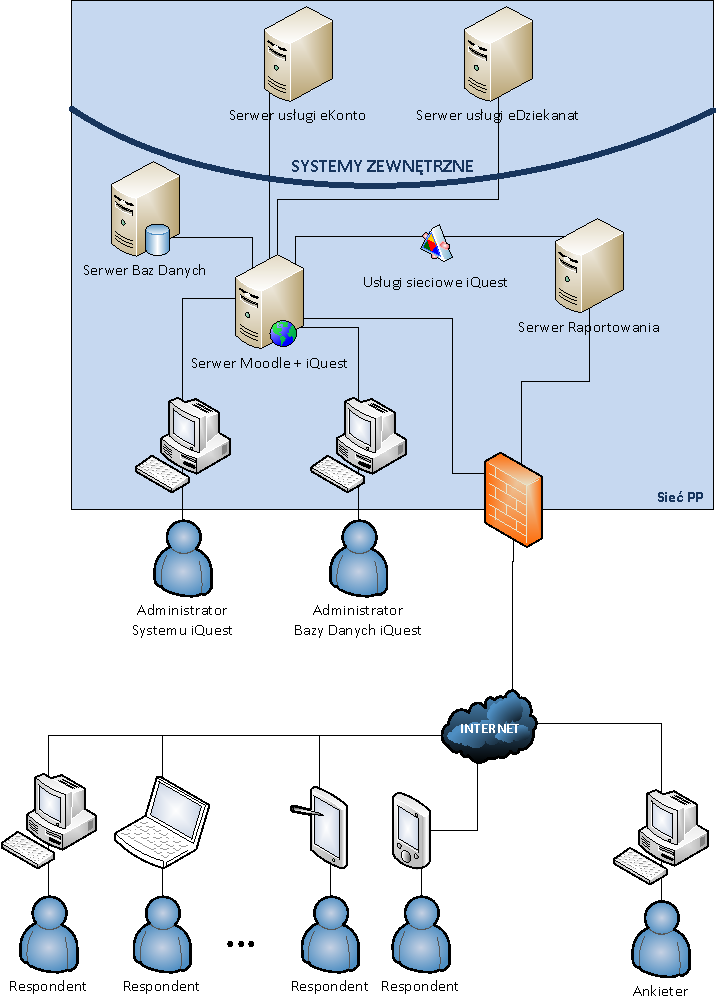
\includegraphics[width=15cm]{figures/marketecture}
\caption{Diagram ,,Marketektury''}\label{rys:marketecture}
\end{figure}

System iQuest to aplikacja internetowa w postaci zbioru rozszerzeń platformy e-learningowej Moodle. Całość (Moodle oraz rozszrzenia) zainstalowana jest na serwerze www, zlokalizowanym w sieci Politechniki Poznańskiej, łączącym się z osobnym serwerem baz danych oraz usługami eKonto i eDziekanat. Funkcje raportowania realizowane są w głównej mierze za pośrednictwem zewnętrznego systemu BI, pobierającego dane z iQuest za pośrednictwem usług sieciowych (en.~\definicja{webservices}). Administracja oraz obsługa systemu odbywa się za pośrednictwem przeglądarki internetowej, w ramach połączenia z platformą Moodle lub serwerem raportowania. Respondenci mogą też uzyskać dostęp do systemu przy pomocy urządzeń mobilnych, takich jak tablety czy smartfony.

%\section{Analiza SWOT}
%\label{Chapter53}
%
%My tego nie mieliśmy, ale chyba warto -- tutaj analiza SWOT przyjętego podejścia architektonicznego.
%
\section{Perspektywy architektoniczne}
\label{Chapter53}

\subsection{Perspektywa fizyczna}
\label{Chapter531}

\begin{figure}[H]
\centering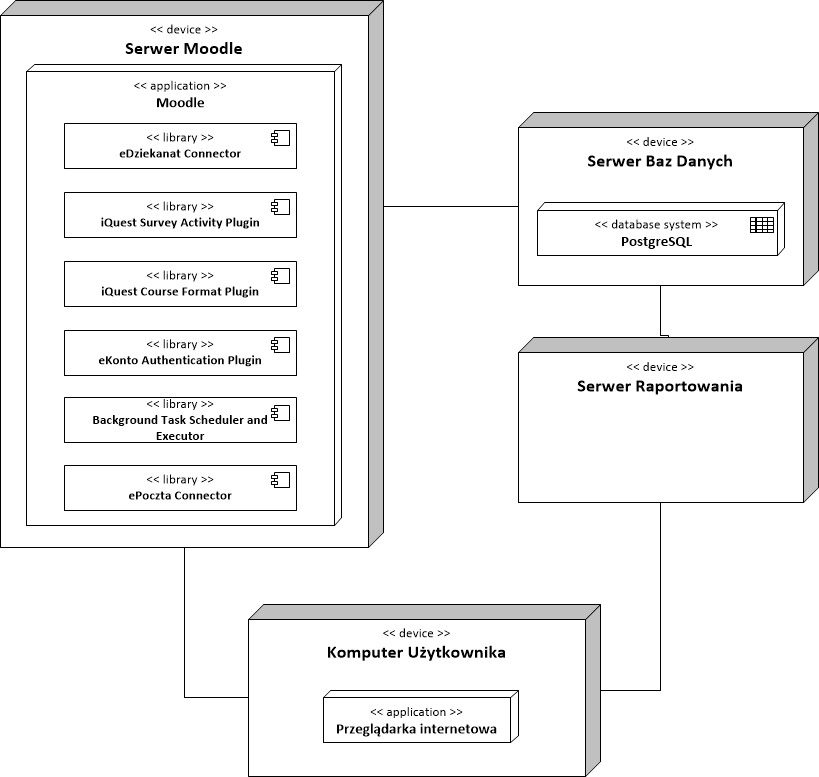
\includegraphics[width=15cm]{figures/PhysicalView}
\caption{Diagram perspektywy fizycznej}\label{rys:PerspektywaFizyczna}
\end{figure}

Powyższy schemat prezentuje perspektywę fizyczną projektu. Widać na nim dokładnie opisaną wcześniej budowę systemu iQuest, opartą na rozszerzeniach dla platformy Moodle, w ramach których wykonywana jest cała logika aplikacji. Za jej pośrednictwem dokonuje on połączeń z serwerem baz danych oraz serwerem raportowania. Użytkownik systemu, z wykorzystaniem przeglądarki internetowej, komunikuje się z platformą, lub systemem raportowania, uzyskując w ten sposób dostęp do warstwy prezentacji.

\subsection{Perspektywa logiczna}
\label{Chapter532}

\begin{figure}[H]
\centering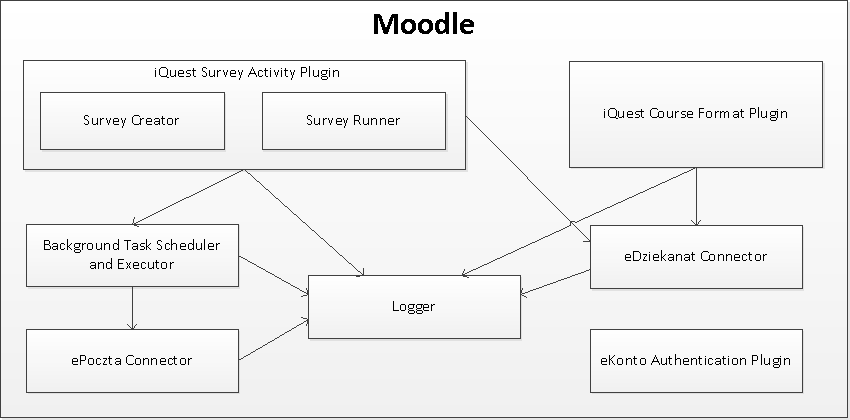
\includegraphics[width=15cm]{figures/LogicalView}
\caption{Diagram perspektywy logicznej}\label{rys:PerspektywaLogiczna}
\end{figure}

Przedstawiony powyżej schemat prezentuje perspektywę logiczną systemu. Określa ona zależności między poszczególnymi komponentami ,,wszczepionymi'' do platformy Moodle. Poniżej znajduje się opis wyszczególnionych na rysunku komponentów.

\subsubsection{iQuest Survey Activity Plugin}
\label{Chapter5321}
Funkcjonalnością Activity Pluginów jest udostępnianie możliwości dodania nowych rodzajów Aktywności w ramach platformy Moodle. Pozwala on na dodanie nowego Badania iQuest w ramach kursu iQuest. Komponent ten składa się z dwóch subkomponentów:
\begin{itemize}
\item{Survey Creator,}
\item{Survey Runner.}
\end{itemize}
Pierwszy z nich odpowiada za definiowanie ankiet, podczas gdy drugi za ich przeprowadzanie.

\subsubsection{iQuest Course Format Plugin}
\label{Chapter5322}

Course Format Plugin dla platformy Moodle odpowiada za obsługę interfejsu użytkownika. W przypadku systemu iQuest, zarządza kwestią wyświetlania użytkownikowi tylko tych składowych kursu "iQuest", które są dla niego dostępne. Przykładowo, Respondent uzyska dostęp do listy ankiet, które może wypełnić, podczas gdy ankieter uzyska dostęp do listy zarządzanych przez niego badań.

\subsubsection{eDziekanat Connector oraz ePoczta Connector}
\label{Chapter5323}

Komponenty te odpowiadają za komunikację z usługami eDziekanat i ePoczta, pozwalające m.in. na pozyskanie danych o grupach docelowych (w oparciu o dane Grup Dziekańskich) oraz wysyłanie powiadomień za pośrednictwem poczty studenckiej.

\subsubsection{Background Task Scheduler and Executor}
\label{Chapter5324}

Dzięki temu komponentowi możliwe jest szeregowanie oraz wykonywanie zadań w tle. Jednym z jego zadań jest kolejkowanie i aktywowanie mechanizmów rozsyłania wiadomości e-mail z zaproszeniami do udziału w ankiecie.

\subsubsection{eKonto Authentication Plugin}
\label{Chapter5325}

eKonto Authentication Plugin -- to moduł uwierzytelniania (ang.~\definicja{Authentication}), korzystający z systemu eLogin platformy eKonto do logowania się do platformy Moodle, obsługującej system iQuest. Korzystanie z tego systemu pozwala nie tylko na jednoznaczną weryfikację tożsamości użytkownika łączącego się z systemem, ale jest zarazem wygodne -- dzięki jego zastosowaniu, nie ma potrzeby posiadania osobnego konta w systemie iQuest.

\subsection{Perspektywa implemetancyjna}
\label{Chapter533}

\begin{figure}[H]
\centering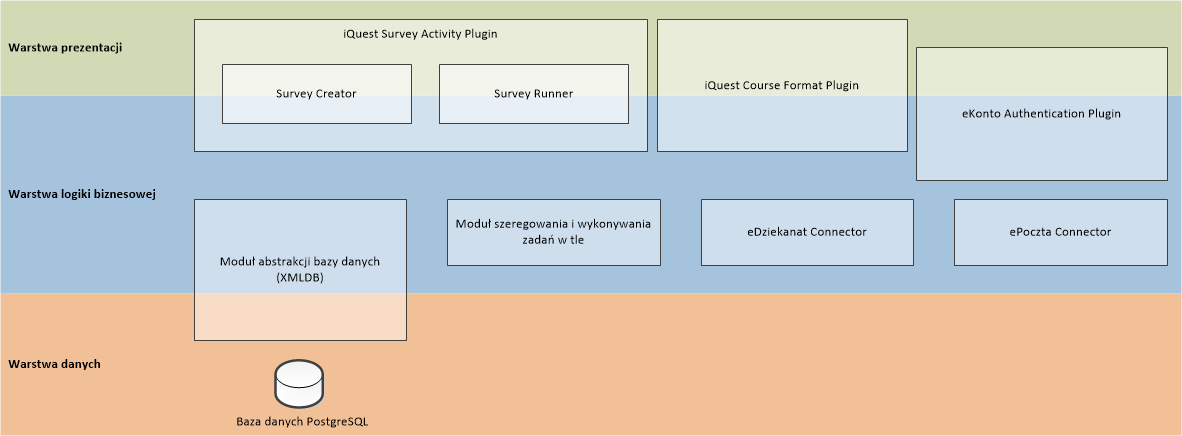
\includegraphics[width=15cm]{figures/Layers}
\caption{Diagram perspektywy implementacyjnej}\label{rys:PerspektywaImplementacyjna}
\end{figure}

Diagram perspektywy implementacyjnej pozwala na analizę przeplatania się elementów systemu iQuest w ramach poszczególnych warstw zastosowanego modelu trójwarstwowego. Funkcje zaprezentowanych na nim modułów zostały wyjaśnione już wcześniej w niniejszym dokumencie.

\subsection{Perspektywa procesu (równoległości)}
\label{Chapter534}

{\color{red}Rysunek wraz z opisem.}

\section{Decyzje projektowe}
\label{Chapter54}

{\color{red}Tutaj będzie o decyzjach projektowych, związkach pomiędzy nimi oraz innych związanych sprawach. Jest tego dość sporo i wymaga specyficznego formatowania.}

\section{Wykorzystane technologie}
\label{Chapter55}

{\color{red}Opis wykorzystywanych technologii (COTS). Sprawdzić czy ten rozdział to nie dubel!}

\section{Schemat bazy danych}
\label{Chapter56}

Schemat bazy danych, ze względu na objętość, zamieszczono w dodatku C.